\section{Dini Permata Putri}
\begin{enumerate}


\item 1. Apa itu fungsi library Matplotlib
Matplotlib adalah sebuah library pada python yang digunakan untuk membuat diagram. Library ini biasanya menghasilkan ploting 2D.\\

Ada plot untuk menampilkan data secara 2D atau 3D. sehingga kamu dapat menampilkan data yang telah kamu olah sesuai kebutuhan. Matplotlib pun terintegrasi dengan ipython notebook atau jupyter dimana kamu dapat membuat sebuah buku interaktif yang dapat diberi penjelasan dan kode yang disisipkan begitupun hasil plottingnya.\\

\item 2. Jelaskan langkah-langkah membuat sumbu X dan Y di matplotlib.
A. Klik kanan scatter chart dan klik pilih data dalam menu konteks , lalu pilih "Select Data

B.Dalam kotak dialog sumber data dan sumber keluar , klik untuk menyoroti Y pada kolom. lalu klik tombol ubah pada tombol di legenda entrl.

C. Sekarang kotak dialog di edit pada series keluar , abis itu silahkan tukar Nilai seri X dan Nilai seri Y lalu klik tombol OK untuk menutup kedua kotak dialog.\\

\item 3. Jelaskan bagaimana perbedaan fungsi dan cara pakai untuk berbagai jenis(bar,histogram,scatter.dll) jenis plot di matloptlib
Untuk perbedaan fungsi plot yang digunakan adalah bentuk bentuk grafik yang akan di tampilkan sesuai dengan perintah yang digunakan pada pemogramannya.\\

line
    Perintah yang digunakan untuk membuat grafik line sebagai berikut.
x = [2,4,6,5,42,543,5,3,73,64,42,97,63,76,63,8,73,97,\\
23,45,56,89,45,3,23,2,5,78,23,56,67,78,8,3,78,34,67,\\
23,324,234,43,544,54,33,223,443,444,234,76,432,233,23,\\
232,243,222,221,254,222,276,300,353,354,387,364,309]\\



Bar itu di dalam Penggunaan plot bar koordinat x nya itu yang awal, dan untuk Y nya adalah yang kedua.\\

Histrogram itu di dalam penggunaan plot histogram titik x nya bisa tidak sama dengan titik Y. untuk penggunaannya bisa sebagai berikut.\\

scatter untuk penggunaa plot scatter atau bisa juga d bilang diagram titik.\\

Stack plot untuk penggunaan stack plot ini seperti diagram line, tapi ada fill colornya,jadi antar line itu bisa berdekatan.\\

\item 4. Jelaskan bagaimana cara menggunakan legend dan label serta kaitannya dengan fungsi tersebut.
Contoh source code lengkap disertai dengan link "editor" untuk mencoba (try it) dan melihat hasil (preview) kode.\\

Elemen yang akan ditambahkan ke legenda ditentukan secara otomatis, ketika Anda tidak memberikan argumen tambahan.\\

Garis-garis spesifik dapat dikecualikan dari pemilihan elemen legenda otomatis dengan mendefinisikan label dimulai dengan garis bawah.\\

\item 5. Jelaskan apa fungsi dari subplot di matplotlib dan fungsi dari subplot dari matplotlib untuk bisa membuat lebih dari 1 grafik dalam sebuah program.\\

Misalnya, kita dapat membuat sumbu inset di sudut kanan atas sumbu lain dengan mengatur posisi x dan y ke 0,65 yaitu, mulai dari 65 peren dari lebar dan 65 persen  dari ketinggian gambar dan x dan y meluas ke 0,2 yaitu, ukuran sumbu adalah 20 persen  dari lebar dan 20persen dari tinggi gambar.\\

Simple Grids of Subplots itu kebutuhan yang cukup umum sehingga Matplotlib memiliki beberapa rutinitas kenyamanan yang membuatnya mudah dibuat. Level terendah adalah plt.subplot (), yang membuat subplot tunggal di dalam kisi. Seperti yang Anda lihat, perintah ini membutuhkan tiga argumen bilangan bulat — jumlah baris, jumlah kolom, dan indeks plot yang akan dibuat dalam skema ini, yang berjalan dari kiri atas ke kanan bawah.\\
Contohnya:\\
for i in range(1, 7):
    plt.subplot(2, 3, i)
    plt.text(0.5, 0.5, str((2, 3, i)),
             fontsize=18, ha='center')
             
The Whole Grid in One Go itu  membuat grid besar subplot, terutama jika Anda ingin menyembunyikan label sumbu x dan y pada plot bagian dalam. Untuk tujuan ini, plt.subplots () adalah alat yang lebih mudah digunakan.\\
 
\item 6. Sebutkan semua parameter color yang bisa digunakan(contoh: m,c,r,k,...dkk)
Tipe Warna RGB
    Untuk keterangannya sebagai berikut
    R untuk warna Red atau Merah
    G untuk warna Green atau Hijau
    B untuk warna Blue atau Biru.\\
    
Tipe warna CMYK
    Untuk keterangannya sebagai berikut
    C untuk warna Cyan atau Biru Muda
    M untuk warna Mangenta atau Merah Tua
    Y untuk warna Yellow Atau Kuning
    K untuk warna blacK atau Hitam.\\

\item 7. Jelaskan bagaimana cara kerja dari fungsi hist , sertakan ilustrasi dan gambar sendiri.
Untuk fungsi histogram ini kedua titik koordinat boleh tidak sama. Misalnya x nya ada 10 nilai sedangkan Y nya ada 5 nilai, itu tidak akan jadi masalah karena diagram ini digunakan untuk mendata usia dari rentang tertentu atau kebutuhan lainnya.\\

Ini merupakan contoh dari penggunaan histogram.\\

\item 8. Jelaskan lebih dalam tentang parameter dari fungsi pie diantaranya labels , color , startangle , shadow , explode , autopct.
Jika jumlah x <1, maka nilai x memberikan area fraksional secara langsung dan array tidak akan dinormalisasi.\\

labels : Label digunakan untuk mempermudah pembaca dalam membaca diagram pie.\\

color : warna digunakan untuk membedakan antar data.\\

startangle : Digunakan untuk sudut yang digunakan untuk memulai diagram pie tersebut.\\

shadow :  bayangan digunakan untuk membuat bayangan dari setiap diagram pie yang menonjol.\\

explode : explode digunakan untuk mengeluarkan suatu data agar data tersebut terlihat menonjol.\\

autopct : Digunakan sesuai dengan berapa angka dibelakang koma yang kita inginkan.\\

\end{enumerate}
%%%%%%%%%%%%%%%%%%%%%%%%%%%%%%%%%%%%%%%%%%%%%%%%%%%%%%%%%%%%%%%%%%%%%%
\section{Advent Nopele Olasni Damiahan Sihite / 1174089}
\subsection{Teori}
\subsubsection{Soal No. 1}
\hfill \break
Apa itu fungsi library matplotlib?

\hfill \break
Matplotlib merupakan salah satu library Python 2D yang dapat menghasilkan plot dengan kualitas yang tinggi dalam berbagai format dan dapat digunakan di berbagai platform. Matplotlib berfungsi sebagai pembuat grafik di berbagai platform, seperti Python dan Jupyter. Grafik yang dibuat menggunakan Matplotlib bisa dibuat dalam berbagai bentuk, seperti grafik garis, batang, lingkaran, histogram, dan sebagainya.

\subsubsection{Soal No. 2}
\hfill \break
Jelaskan langkah-langkah membuat sumbu X dan Y di matplotlib!

\begin{enumerate}
	\item Pertama import library Matplotlib.	
	\lstinputlisting[firstline=2, lastline=2]{src/6/1174089/Teori/1174089.py}
	
	\item Buat variabel x yang menampung list untuk sumbu x dan variabel y yang menampung list untuk sumbu y.	
	\lstinputlisting[firstline=4, lastline=5]{src/6/1174089/Teori/1174089.py}
	
	\item Panggil fungsi plot dan isi parameter pertama dengan variabel x dan parameter kedua dengan variabel y.
	\lstinputlisting[firstline=7, lastline=7]{src/6/1174089/Teori/1174089.py}	

	\item Lalu panggil plot tadi dengan memanggil fungsi show.
	\lstinputlisting[firstline=9, lastline=9]{src/6/1174089/Teori/1174089.py}
	
\end{enumerate}
\hfill \break
\textbf{Kode Program}

\lstinputlisting[caption = Kode program membuat diagram menggunakan Matplotlib., firstline=2, lastline=9]{src/6/1174089/Teori/1174089.py}

\hfill \break
\textbf{Hasil Compile}

\begin{figure}[H]
	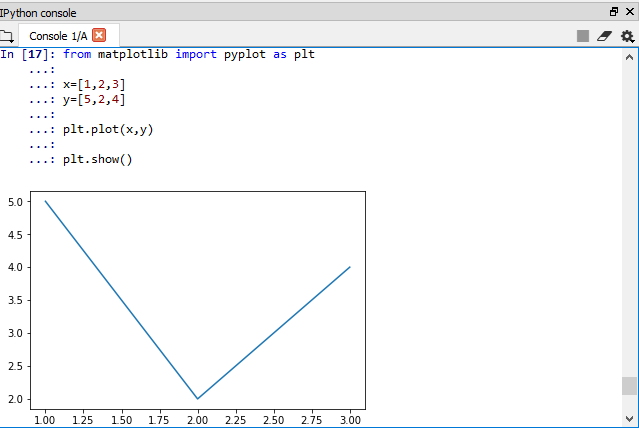
\includegraphics[width=12cm]{figures/6/1174089/Teori/2.png}
	\centering
	\caption{Hasil compile membuat diagram menggunakan Matplotlib.}
\end{figure}
 
\subsubsection{Soal No. 3}
\hfill \break
Jelaskan bagaimana perbedaan fungsi dan cara pakai untuk berbagai jenis(bar, histogram ,scatter ,line, dll) jenis plot di matplotlib!

\begin{enumerate}
	\item \textbf{Bar Graph}
	
	Perbedaan bar graph dengan jenis plot yang lain adalah bar graph menggunakan bar atau batang-batang untuk membandingkan data di antara berbagai kategori.
	
	\textbf{Kode Program}
	
	\lstinputlisting[caption = Kode program membuat bar graph menggunakan Matplotlib., firstline=2, lastline=9]{src/6/1174089/Teori/1174089.py}
	
	\textbf{Hasil Compile}
	
	\begin{figure}[H]
		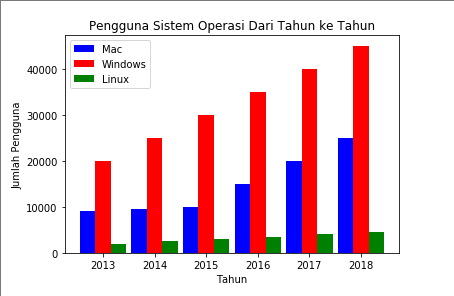
\includegraphics[width=12cm]{figures/6/1174089/Teori/bar.png}
		\centering
		\caption{Hasil compile membuat bar graph menggunakan Matplotlib.}
	\end{figure}
	
	\item \textbf{Histogram}
	
	Perbedaan histogram dengan jenis plot yang lain adalah histogram akan membuat plot dimana plot yang dimunculkan merupakan gabungan dari beberapa data yang telah dikelompokkan.
	
	\textbf{Kode Program}
	
	\lstinputlisting[caption = Kode program membuat histogram menggunakan Matplotlib., firstline=29, lastline=36]{src/6/1174089/Teori/1174089.py}
	
	\textbf{Hasil Compile}
	
	\begin{figure}[H]
		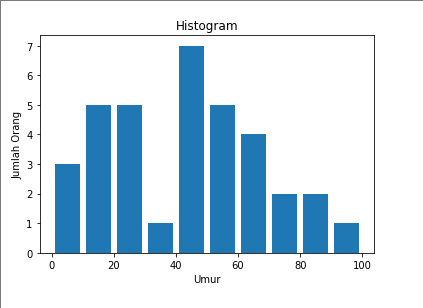
\includegraphics[width=12cm]{figures/6/1174089/Teori/histogram.png}
		\centering
		\caption{Hasil compile membuat histogram menggunakan Matplotlib.}
	\end{figure}
	
	\item \textbf{Scatter Plot}
	
	Perbedaan scatter plot dengan jenis plot lain adalah scatter plot menampilkan data sebagai kumpulan titik, masing-masing memiliki nilai satu variabel yang menentukan posisi pada sumbu horizontal dan nilai variabel lain menentukan posisi pada sumbu vertikal.
	
	\textbf{Kode Program}
	
	\lstinputlisting[caption = Kode program membuat scatter plot menggunakan Matplotlib., firstline=40, lastline=53]{src/6/1174089/Teori/1174089.py}
	
	\textbf{Hasil Compile}
	
	\begin{figure}[H]
		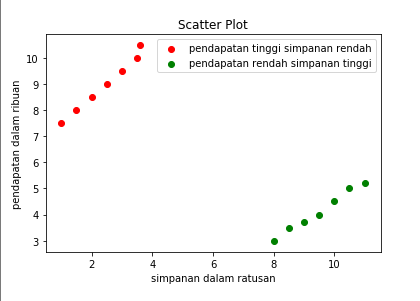
\includegraphics[width=12cm]{figures/6/1174089/Teori/scatter.png}
		\centering
		\caption{Hasil compile membuat scatter plot menggunakan Matplotlib.}
	\end{figure}
	
	\item \textbf{Area Plot}
	
	Perbedaan area plot dengan jenis plot lain adalah area plot digunakan untuk melacak perubahan dari waktu ke waktu untuk dua atau lebih kelompok terkait yang membentuk satu kategori secara keseluruhan.
	
	\textbf{Kode Program}
	
	\lstinputlisting[caption = Kode program membuat diagram menggunakan Matplotlib., firstline=57, lastline=76]{src/6/1174089/Teori/1174089.py}
	
	\textbf{Hasil Compile}
	
	\begin{figure}[H]
		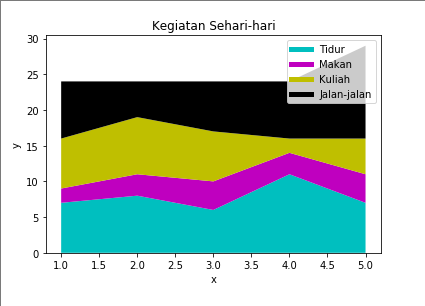
\includegraphics[width=12cm]{figures/6/1174089/Teori/area.png}
		\centering
		\caption{Hasil compile membuat diagram menggunakan Matplotlib.}
	\end{figure}
	
	\item \textbf{Pie Plot}
	
	Perbedaan pie plot dengan jenis plot lain adalah pie plot digunakan untuk menunjukkan persentase atau data proporsional di mana setiap potongan pie mewakili kategori.
	
	\textbf{Kode Program}
	
	\lstinputlisting[caption = Kode program membuat Pie Plot menggunakan Matplotlib., firstline=80, lastline=101]{src/6/1174089/Teori/1174089.py}
	
	\textbf{Hasil Compile}
	
	\begin{figure}[H]
		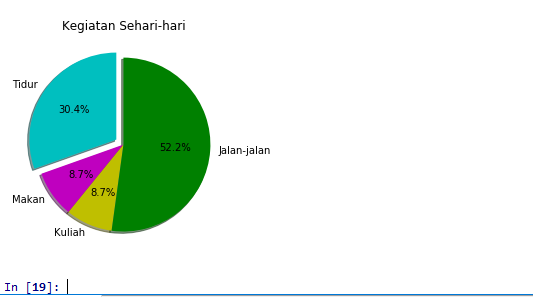
\includegraphics[width=9cm]{figures/6/1174089/Teori/pie.png}
		\centering
		\caption{Hasil compile membuat Pie Plot menggunakan Matplotlib.}
	\end{figure}
	
	\item \textbf{Line Graph}
	
	Perbedaan line graph dengan jenis plot lain adalah line graph menampilkan diagram dalam bentuk garis.
	
	\textbf{Kode Program}
	
	\lstinputlisting[caption = Kode program membuat diagram menggunakan Matplotlib., firstline=105, lastline=113]{src/6/1174089/Teori/1174089.py}
	
	\textbf{Hasil Compile}
	
	\begin{figure}[H]
		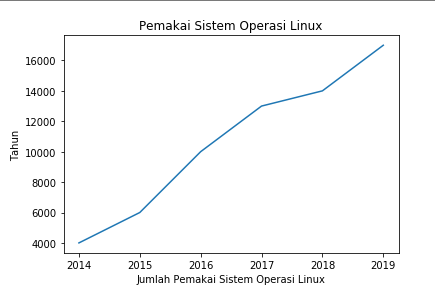
\includegraphics[width=12cm]{figures/6/1174089/Teori/line.png}
		\centering
		\caption{Hasil compile membuat diagram menggunakan Matplotlib.}
	\end{figure}
	
\end{enumerate}

\subsubsection{Soal No. 4}
\hfill \break
Jelaskan bagaimana cara menggunakan legend dan label serta kaitannya dengan fungsi tersebut!

\begin{enumerate}
	\item Untuk menggunakan legend definisikan parameter label di tiap fungsi plot. Parameter label digunakan untuk memberikan label pada line sebagai pembeda antar line.
	
	\lstinputlisting[caption = Kode program menggunakan parameter label dengan Matplotlib., firstline=123, lastline=124]{src/6/1174089/Teori/1174089.py}
	
	\item Kemudian panggil fungsi legend.
	
	\lstinputlisting[caption = Kode program memanggil fungsi legend dengan Matplotlib., firstline=128, lastline=128]{src/6/1174089/Teori/1174089.py}
\end{enumerate}

\hfill \break
\textbf{Kode Program}

\lstinputlisting[caption = Kode program membuat diagram menggunakan Matplotlib., firstline=117, lastline=130]{src/6/1174089/Teori/1174089.py}

\hfill \break
\textbf{Hasil Compile}

\begin{figure}[H]
	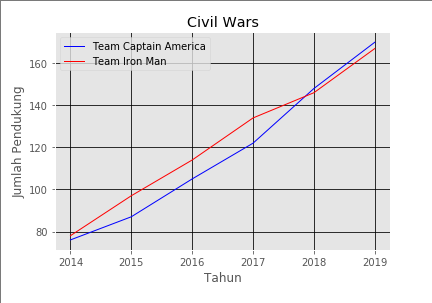
\includegraphics[width=12cm]{figures/6/1174089/Teori/4.png}
	\centering
	\caption{Hasil compile membuat diagram menggunakan Matplotlib.}
\end{figure}

\subsubsection{Soal No. 5}
\hfill \break
Jelaskan apa fungsi dari subplot di matplotlib, dan bagaimana cara kerja dari fungsi subplot, sertakan ilustrasi dan gambar sendiri dan apa parameternya jika ingin menggambar plot dengan 9 subplot di dalamnya!

\hfill \break
Fungsi subplot adalah untuk membuat beberapa plot di dalam satu gambar.
\hfill \break
Cara kerja subplot, yaitu fungsi subplot memiliki parameter pertama adalah jumlah kolom, parameter kedua adalah jumlah baris, dan parameter ketiga adalah index plot keberapanya.

\hfill \break
\textbf{Kode Program}

\lstinputlisting[caption = Kode program membuat subplot menggunakan Matplotlib., firstline=134, lastline=146]{src/6/1174089/Teori/1174089.py}

\hfill \break
\textbf{Hasil Compile}

\begin{figure}[H]
	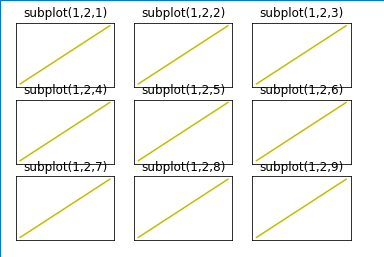
\includegraphics[width=12cm]{figures/6/1174089/Teori/subplot.png}
	\centering
	\caption{Hasil compile membuat subplot menggunakan Matplotlib.}
\end{figure}

\subsubsection{Soal No. 6}
\hfill \break
Sebutkan semua parameter color yang bisa digunakan (contoh:  m,c,r,k,...  dkk)!

\begin{itemize}
	\item 'b' (blue)
	\item 'g' (green)
	\item 'r' (red)
	\item 'c' (cyan)
	\item 'm' (magenta)
	\item 'y' (yellow)
	\item 'k' (black)
	\item 'w' (white)
\end{itemize}

\subsubsection{Soal No. 7}
\hfill \break
Jelaskan bagaimana cara kerja dari fungsi hist, sertakan ilustrasi dan gambar sendiri!

\hfill \break
Cara kerja dari fungsi hist yaitu fungsi hist akan menerima parameter yang diberikan, kemudian fungsi hist akan dieksekusi sesuai dengan parameter yang diberikan.

\hfill \break
\textbf{Kode Program}

\lstinputlisting[caption = Kode program membuat diagram menggunakan Matplotlib., firstline=150, lastline=157]{src/6/1174089/Teori/1174089.py}

\hfill \break
\textbf{Hasil Compile}

\begin{figure}[H]
	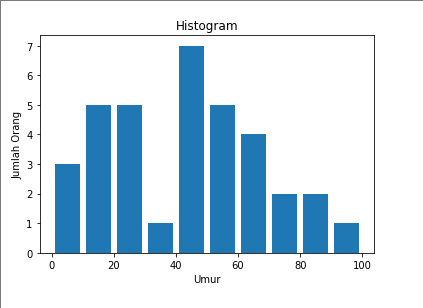
\includegraphics[width=12cm]{figures/6/1174089/Teori/histogram.png}
	\centering
	\caption{Hasil compile membuat diagram menggunakan Matplotlib.}
\end{figure}

\subsubsection{Soal No. 8}
\hfill \break
 Jelaskan lebih mendalam tentang parameter dari fungsi pie diantaranya labels, colors, startangle, shadow, explode, autopct!
 
 \begin{itemize}
 	\item labels : untuk memberikan label di tiap persentase.
 	\item colors : untuk memberikan warna di tiap persentase.
 	\item startangle : untuk memutar plot sesuai dengan derajat yang ditentukan.
 	\item shadow : untuk memberikan bayangan pada plot.
 	\item explode : untuk memisahkan antar tiap potongan pie pada plot.
 	\item autopct : untuk menentukan jumlah angka dibelakang koma.
 \end{itemize}

\subsection{Praktek}
\subsubsection{Soal No. 1}
\hfill \break
Buatlah librari fungsi (file terpisah/library dengan nama NPMbar.py) untuk plot dengan jumlah subplot adalah NPM mod 3 + 2!

\subsubsection{Soal No. 2}
\hfill \break
Buatlah librari fungsi (file terpisah/library dengan nama NPMscatter.py) untuk plot dengan jumlah subplot NPM mod 3 + 2!

\subsubsection{Soal No. 3}
\hfill \break
Buatlah librari fungsi (file terpisah/library dengan nama NPMpie.py) untuk plot dengan jumlah subplot NPM mod 3 + 2!

\subsubsection{Soal No. 4}
\hfill \break
Buatlah librari fungsi (file terpisah/library dengan nama NPMplot.py) untuk plot dengan jumlah subplot NPM mod 3 + 2


\subsection{Penanganan Error}
Tuliskan  peringatan  error  yang  didapat  dari  mengerjakan  praktek  keenam  ini, dan  jelaskan  cara  penanganan  error  tersebut. dan  Buatlah  satu  fungsi  yang menggunakan try except untuk menanggulangi error tersebut.
%%%%%%%%%%%%%%%%%%%%%%%%%%%%%%%%%%%%%%%%%%%%%%%%%%%%%%%%%%%%%
\section{Bakti Qilan Mufid | 1174083}
\subsection{Teori}
\subsubsection{Apa itu fungsi library matplotlib}
\hfill \break
\verb|matplotlib| adalah librari plotting 2D Python yang menghasilkan gambar publikasi bermutu di dalam berbagai format hardcopy dan lingkungan interaktif sepanjang platform. \verb|matplotlib| dapat digunakan di dalam script Python, shell Python dan ipython (ala MATLAB®* or Mathematica®), server aplikasi web, dan enam GUI toolkit. matplotlib mencoba untuk membuat hal mudah menjadi lebih mudah dan hal sulit menjadi mungkin. Kamu dapat membuat plot, histogram, power spectra, grafik batang, grafik error, scatterplot, dll, hanya dengan beberapa baris code.

\subsubsection{Jelaskan langkah-langkah membuat sumbu X dan Y di matplotlib}
\hfill \break
Untuk membuat sumbu X dan Y kita bisa membuatnya menggunakan list untuk mempermudah penyimpanan nilai pada setiap sumbunya. seperti pada contoh berikut:
\lstinputlisting[firstline=11, lastline=19]{src/6/1174083/Teori/1174083.py}

maka ketika di run akan menghasilkan diagram sebagai beriku:
\begin{figure}[ht]	
    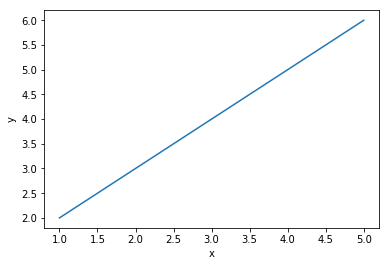
\includegraphics[width=4cm]{figures/6/1174083/Teori/1.png}
    \centering
    \caption{penjelasan membuat sumbu x dan y}
    \label{1}
\end{figure}

\subsubsection{Jelaskan bagaimana perbedaan fungsi dan cara pakai untuk berbagai jenis(bar,histogram,scatter,line dll) jenis plot di matplotlib}
\hfill \break
Macam-macam plot di matplotlib, diantaranya:
\begin{enumerate}
\item Plot Garis \hfill \break
Diagram Garis (\textit{Line Chart}) digunakan untuk melihat trend/ pergerakan suatu variabel data tertentu. Diagram garis juga dapat disebut sebagai diagram runtun waktu atau \textit{Time Series Plot}. dan cara pakai Plot Garis ini seperti pada kode berikut:
\lstinputlisting[firstline=23, lastline=31]{src/6/1174083/Teori/1174083.py}
\begin{figure}[ht]	
    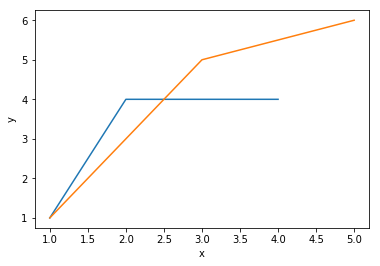
\includegraphics[width=4cm]{figures/6/1174083/Teori/2.png}
    \centering
    \caption{contoh Plot Garis}
    \label{2}
\end{figure}
\newpage
\item Plot Sebaran atau Scatter Plot \hfill \break
adalah sebuah grafik yang menunjukkan hubungan antara dua set data. dan cara pakai Plot Sebaran atau Scatter ini seperti pada kode berkut:
\lstinputlisting[firstline=35, lastline=43]{src/6/1174083/Teori/1174083.py}
\begin{figure}[ht]	
    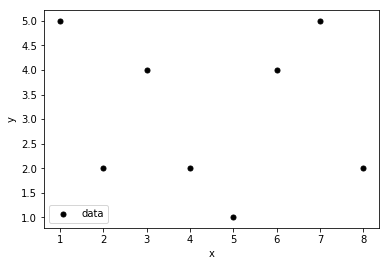
\includegraphics[width=4cm]{figures/6/1174083/Teori/3.png}
    \centering
    \caption{contoh Plot Scatter}
    \label{3}
\end{figure}

\item Histogram \hfill \break
adalah grafik yang menampilkan frekuensi data menggunakan batang, dimana angka dikelompokkan dalam rentang tertentu. Dengan kata lain, frekuensi setiap elemen data di dalam daftar ditunjukkan menggunakan histogram. Angka yang dikelompokkan dalam bentuk rentang tertentu disebut \textit{bins}. Untuk cara penggunaanya seperti pada kode berikut:
\lstinputlisting[firstline=46, lastline=53]{src/6/1174083/Teori/1174083.py}
\begin{figure}[ht]	
    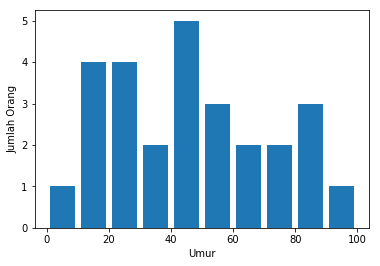
\includegraphics[width=4cm]{figures/6/1174083/Teori/4.png}
    \centering
    \caption{contoh Histogram}
    \label{4}
\end{figure}

\item Bar \hfill \break
Diagram Batang (\textit{bar Chart}) adalah diagram yang menggambarkan data dengan menggunakan batang vertikal atau horizontal yang memiliki tinggi atau panjang yang menunjukan frekuensi data. untuk pemakainannya seperti pada kode berikut:
\lstinputlisting[firstline=56, lastline=66]{src/6/1174083/Teori/1174083.py}
\begin{figure}[ht]	
    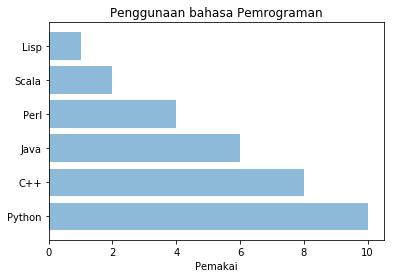
\includegraphics[width=5cm]{figures/6/1174083/Teori/5.png}
    \centering
    \caption{contoh Bar}
    \label{5}
\end{figure}
\end{enumerate}

\subsubsection{Jelaskan bagaimana cara menggunakan legend dan label serta kaitannya dengan fungsi tersebut}
\hfill \break
Legend merupakan bagian dalam grafik yang isinya adalah keterangan dari grafik tersebut. dan label ialah untuk penamaan pada grafik tersebut. Dan cara menggunakan Legend dan lebel cukup mudah, seperti pada kode berikut:
\lstinputlisting[firstline=40, lastline=42]{src/6/1174083/Teori/1174083.py}
contohnya ada pada \textbf{gambar 1.3} dimana legend berada pada pojok kiri bawah, dan dan contoh labelnya x dan y.

\subsubsection{Jelaskan apa fungsi dari subplot di matplotlib, dan bagaimana cara kerja dari fungsi subplot, sertakan ilustrasi dan gambar sendiri dan apa parameternya jika ingin menggambar plot dengan 9 subplot di dalamnya}
\hfill \break
Fungsi subplot di matplotlib ialah untuk menggabungkan beberapa grafik menjadi satu figure. dan cara kerja dari fungsi subplot ini bisa dilihat pada kode berikut:
\lstinputlisting[firstline=69, lastline=81]{src/6/1174083/Teori/1174083.py}
\begin{figure}[ht]	
    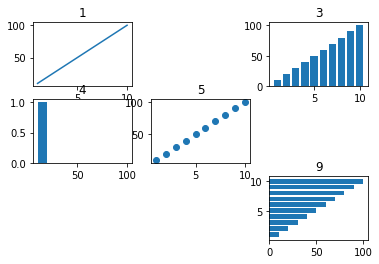
\includegraphics[width=10cm]{figures/6/1174083/Teori/6.png}
    \centering
    \caption{contoh Subplot}
    \label{5}
\end{figure}
\subsubsection{Sebutkan semua parameter color yang bisa digunakan (contoh: m,c,r,k,... dkk)}
\hfill \break
Untuk Nama-nama parameter yang basic seperti pada RGB dan CYMK bisa digunakan seperti berikut:
\begin{itemize}
\item R untuk Red atau Merah
\item G untuk Green atau Hijau
\item B untuk Blue atau Biru
\item C untuk Cyan atau Biru Muda
\item Y untuk Yellow atau Kuning
]item M untuk Magenta atau Merah Tua
\item K untuk Black atau Hitam
\end{itemize}
dan Berikut merupakan daftar warna yang ada pada matplotlib
\begin{figure}[ht]	
    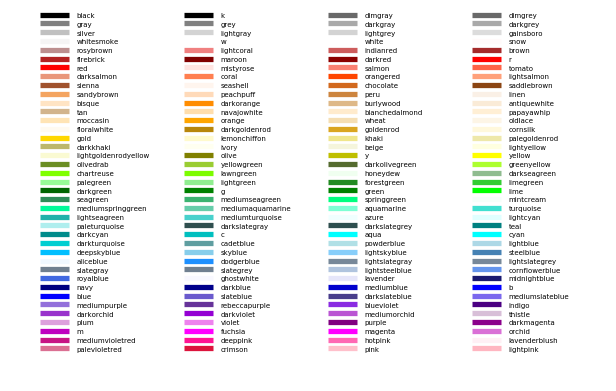
\includegraphics[width=13cm]{figures/6/1174083/Teori/warna.png}
    \centering
    \caption{Daftar warna}
    \label{6}
\end{figure}

\subsubsection{Jelaskan bagaimana cara kerja dari fungsi hist, sertakan ilustrasi dan gambar sendiri}
\hfill \break
Untuk histogram kita tidak boleh memiliki isi variable x dan y yang sama. Misal x-nya ada 10 nilai sedangkan Y-nya ada 5 nilai, data tersebut tidak menjadi masalah karena pada histogram data yang dimunculkan adalah data rentang dari data variable y. Dan ini adalah contoh dari penggunaan histogram

\lstinputlisting[firstline=134, lastline=138]{src/6/1174083/Teori/1174083.py}
\begin{figure}[ht]	
    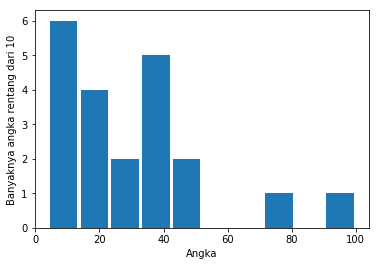
\includegraphics[width=4cm]{figures/6/1174083/Teori/7.png}
    \centering
    \caption{cara kerja fungsi hist}
    \label{6}
\end{figure}
\newpage
\subsubsection{Jelaskan lebih mendalam tentang parameter dari fungsi pie diantaranya labels, colors, startangle, shadow, explode, autopct}
\begin{enumerate}
\item Labels Label digunakan untuk mempermudah pembaca dalam membaca diagram pie
\item Colors  warna digunakan untuk membedakan antar data
\item Statangle digunakan untuk sudut yang berguna untuk memulai diagram pie tersebut
\item Shadow digunakan untuk membuat bayangan dari setiap diagram pie yang menonjol
\item Explode digunakan untuk mengeluarkan suatu data agar data tersebut terlihat menonjol
\item Autobot digunakan sesuai dengan berapa angka dibelakang koma yang kita inginkan
\end{enumerate}
%%%%%%%%%%%%%%%%%%%%%%%%%%%%%%%%%%%%%%%%%%%%%%%%%%%%%%%%%%%%%%%%%%%%%%%%%%%%%%%%%%%%%%%%%%%%%%
\section{Ilham Muhammad Ariq}
\subsection{Pemahaman Teori}
\begin{enumerate}
\item Apa itu fungsi library matplotlib

	Matplotlib adalah sebuah library plotting 2D Python yang menghasilkan gambar publikasi bermutu didalam berbagai format hardcopy dan lingkungan interaktif sepanjang platform. Matplotlib bisa digunakan didalam sebuah script Python, shell Python dan ipython (ala MATLAB®* or Mathematica®), server aplikasi web, dan enam GUI toolkit. Matplotlib mencoba untuk membuat hal yang mudah menjadi lebih mudah dan hal yang sulit menjadi mungkin. Dengan matplotlib,dapat membuat plot, histogram, power spectra, grafik batang, grafik error, scatterplot, dll, hanya dengan beberapa baris code.

\item Jelaskan langkah-langkah membuat sumbu X dan Y di matplotlib
\begin{enumerate}
	\item pertama import dulu library matplotlib lalu beri alias plt
	\lstinputlisting[firstline=8, lastline=8]{src/6/1174087/Teori/1174087_matplotlib.py}

	\item Kemudian buat variable array x dengan isi terserah anda
	\lstinputlisting[firstline=9, lastline=9]{src/6/1174087/Teori/1174087_matplotlib.py}

	\item Lalu buat variable array y juga dengan isi terserah anda yang penting jumlahnya sama dengan variable X
	\lstinputlisting[firstline=10, lastline=10]{src/6/1174087/Teori/1174087_matplotlib.py}

	\item Kemudian buat plot berisikan variable x dan y pada modul plt
	\lstinputlisting[firstline=11, lastline=11]{src/6/1174087/Teori/1174087_matplotlib.py}

	\item Yang terakhir, munculkan plot yang telah kita buat dengan fungsi show()
	\lstinputlisting[firstline=12, lastline=12]{src/6/1174087/Teori/1174087_matplotlib.py}
\end{enumerate}

\item Jelaskan bagaimana perbedaan fungsi dan cara pakai untuk berbagai jenis(bar,histogram,scatter,line dll) jenis plot di matplotlib

Perbedaan pada fungsi plot adalah pada bentuk gambar grafik yang dihasilkan pada program dan jenis jenis grafik yang ada pada plot adalah:
\begin{itemize}
	\item Plot

	Grafik yang dihasilkan adalah sebuah garis 
	\lstinputlisting[firstline=8, lastline=12]{src/6/1174087/Teori/1174087_matplotlib.py}

	\item Bar

	Grafik yang dihasilkan adalah sebuah bentuk grafik batang
	\lstinputlisting[firstline=15, lastline=19]{src/6/1174087/Teori/1174087_matplotlib.py}

	\item Histogram

	grafik yang menampilkan sebuah frekuensi data menggunakan batang/bar , dimana angka dikelompokkan dalam rentang tertentu
	\lstinputlisting[firstline=22, lastline=25]{src/6/1174087/Teori/1174087_matplotlib.py}

	\item Scatter

	Grafik yang dihasilkan diagram titik 
	\lstinputlisting[firstline=28, lastline=39]{src/6/1174087/Teori/1174087_matplotlib.py}
\end{itemize}

	\item  Jelaskan bagaimana cara menggunakan legend dan label serta kaitannya dengan fungsi tersebut

	Untuk menggunakan legend definisikan parameter label di tiap fungsi plot. Parameter label digunakan untuk memberikan label pada line sebagai pembeda antar line.
	\lstinputlisting[firstline=33, lastline=38]{src/6/1174087/Teori/1174087_matplotlib.py}
	
	\item Jelaskan apa fungsi dari subplot di matplotlib, dan bagaimana cara kerja dari fungsi subplot, sertakan ilustrasi dan gambar sendiri dan apa parameternya jika ingin menggambar plot dengan 9 subplot di dalamnya
	
	\par Fungsi subplot adalah untuk membuat beberapa plot di dalam satu gambar.
	\par Cara kerja subplot, yaitu fungsi subplot memiliki parameter pertama adalah jumlah kolom, parameter kedua adalah jumlah baris, dan parameter ketiga adalah index plot keberapanya.	
	
	\lstinputlisting[firstline=42, lastline=62]{src/6/1174087/Teori/1174087_matplotlib.py}
	
	\item Sebutkan semua parameter color yang bisa digunakan (contoh: m,c,r,k,... dkk)
	
	\begin{itemize}
	\item 'b' (blue) = biru
	\item 'g' (green) = hijau
	\item 'r' (red) = merah
	\item 'c' (cyan) = biru muda
	\item 'm' (magenta) = marron 
	\item 'y' (yellow) = kuning
	\item 'k' (black) = hitam
	\item 'w' (white) = putih
	\end{itemize}
		
	\item Jelaskan bagaimana cara kerja dari fungsi hist, sertakan ilustrasi dan gambar sendiri		
	
	\par Untuk histogram variable x dan y tidak ada yang sama. Misal X nya ada 10 angka sedangkan Y nya ada 2 nilai, data tersebut tidak akan error karena pada histogram data yang dimunculkan adalah data rentang dari data variable y. Dan ini adalah contoh program :
	
		\lstinputlisting[firstline=22, lastline=25]{src/6/1174087/Teori/1174087_matplotlib.py}
	
	\item Jelaskan lebih mendalam tentang parameter dari fungsi pie diantaranya labels, colors, startangle, shadow, explode, autopct

\begin{itemize}
    \item \textbf{Label}
    Label digunakan untuk mempermudah pembaca yaitu memberikan nama pada variable di grafik

    \item \textbf{Color}
    Warna yang dimunculkan pada setiap data

    \item \textbf{Startangle}
    Startangle digunakan untuk sudut awal pada diagram pie tersebut

    \item \textbf{Shadow}
    Shadow(Bayangan) digunakan untuk membuat bayangan pada setiap diagram pie yang menonjol

    \item \textbf{Explode}
    Explode digunakan untuk mengeluarkan suatu data agar data tersebut menjadi terlihat lebih menonjol

    \item \textbf{Autopct}
    Autopct digunakan menyesuaikan berapa angka yang ada dibelakang koma
\end{itemize}
\end{enumerate}

\textbf{Screenshoot Plagiarisme}
\begin{figure}[ht]	
    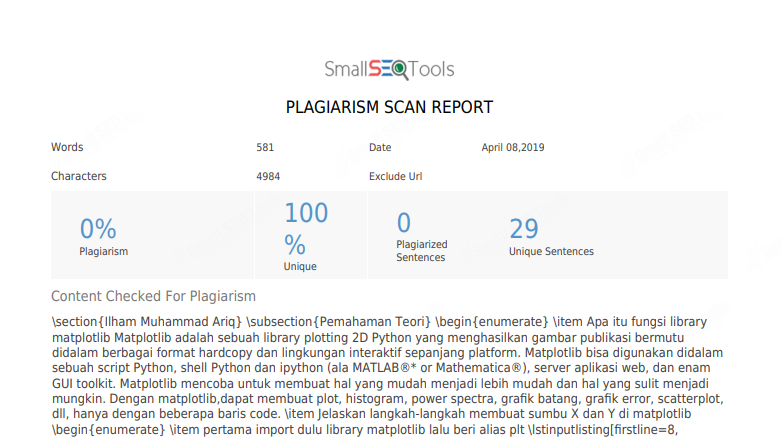
\includegraphics[width=7cm]{figures/6/1174087/Teori/plg.png}
    \centering
    \caption{Screenshoot Plagiarisme}
\end{figure}
%%%%%%%%%%%%%%%%%%%%%%%%%%%%%%%%%%%%%%%%%%%%%%%%%%%%%%%%%%%%%%%%%%%%%%%%%%%%%%%%%%%%%%%%%%%%%%%%%%%%%%%%

\section{Muhammad Reza Syachrani / 1174084}
\subsection{Pemahaman Teori}
\begin{enumerate}
    \item Matplotlib adalah library plotting 2D Python yang menghasilkan gambar. Matplotlib dapat membuat plot, histogram, power spectra, grafik batang, grafik error, scatterplot, dll, dengan beberapa baris code pada python.
    \item langkah-langkah membuat sumbu X dan Y di matplotlib :
    \begin{itemize}
        \item mengimport pyplot dari library matplotlib
        \item menentukan nilai sumbu x dan y pada variable menggunakan list
        \lstinputlisting[firstline=8, lastline=14,]{src/6/1174084/Teori/1174084.py}
    \end{itemize}
    \item Perbedaan fungsi dan cara pakai untuk berbagai jenis (bar, histogram, scatter, line, dll) plot di matplotlib :
    \begin{itemize}
        \item Bar berfungsi menampilkan grafik yang frekunsi data menggunakan batang, yang nilai koordinat x dan y ditentukan. Dalam penggunaan plot bar menggunakan fungsi bar yang terdapat dalam pyplot
        \lstinputlisting[firstline=16, lastline=25,]{src/6/1174084/Teori/1174084.py}
        \item Histogram berfungsi menampilkan grafik yang frekuensi data menggunakan batang, dimana nilai dikelompokkan dalam rentang tertentu dan  Dalam penggunaan plot histogram menggunakan fungsi hist yang terdapat dalam pyplot 
        \lstinputlisting[firstline=27, lastline=35,]{src/6/1174084/Teori/1174084.py}
        \item Scatter berfungsi menampilkan grafik yang menunjukkan hubungan antara dua set nilai menggunakan titik-titik dan Dalam penggunaan plot scatter menggunakan fungsi scatter yang terdapat dalam pyplot
        \lstinputlisting[firstline=8, lastline=14,]{src/6/1174084/Teori/1174084.py}
        \item Line berfungsi menampilkan grafik dari dua set nilai yang menggunakan garis.
        \lstinputlisting[firstline=37, lastline=47,]{src/6/1174084/Teori/1174084.py}
    \end{itemize}
    \item Cara menggunakan legend adalah payplot.legend() dan menambahkan labelnya seperti dibawah ini:
    \lstinputlisting[firstline=21, lastline=23,]{src/6/1174084/Teori/1174084.py}
    Penggunaan legend berfungsi untuk memudahkan kita membaca grafik yang kita hasilkan karena kita memberi informasi pada data yang ditampilkan. sedangkan label kita memberikan nama kepada variable yang membedakan antara variable yang satu dengan yang lain.
    \item fungsi dari subplot di matplotlib adalah untuk bisa membuat lebih dari 1 grafik dalam sebuah program. Cara penggunaannya sebagai contoh berikut :
    \lstinputlisting[firstline=49, lastline=73,]{src/6/1174084/Teori/1174084.py}
    \item Parameter warna yang bisa digunakan :
    \begin{itemize}
        \item R untuk warna Red atau Merah
        \item G untuk warna Green atau Hijau
        \item B untuk warna Blue atau Biru
        \item C untuk warna Cyan atau Biru Muda
        \item M untuk warna Mangenta atau Merah Tua
        \item Y untuk warna Yellow Atau Kuning
        \item K untuk warna Black atau Hitam
    \end{itemize}
    \item Cara kerja dari fungsi histogram boleh memiliki jumlah data variabel yang tidak sama. Contohnya  nilai x nya ada 60 sedangkan nilai Y nya ada 6 nilai, itu tidak akan jadi masalah karena diagram ini digunakan untuk mendata dari rentang tertentu atau kebutuhan lainnya. Dan ini adalah contoh dari penggunaan histogram :
    \lstinputlisting[firstline=27, lastline=35,]{src/6/1174084/Teori/1174084.py}
    \item Jelaskan lebih mendalam tentang parameter dari fungsi pie diantaranya labels,colors, startangle, shadow, explode, autopct
    \begin{itemize}
    \item Label
    Label digunakan untuk mempermudah pembaca yaitu memberikan nama pada variable di diagram pie
    \item Color merupakan Warna yang dimunculkan pada setiap data
    \item Startangle digunakan untuk sudut awal pada diagram pie tersebut
    \item Shadow
    Shadow(Bayangan) digunakan untuk membuat bayangan pada setiap diagram pie yang menonjol
    \item Explode digunakan untuk mengeluarkan suatu data agar data tersebut menjadi terlihat lebih menonjol
    \item Autopct digunakan menyesuaikan berapa angka yang ada dibelakang koma
    \end{itemize}
    \item Scan Plagiarisme
    \begin{figure}[ht!]
    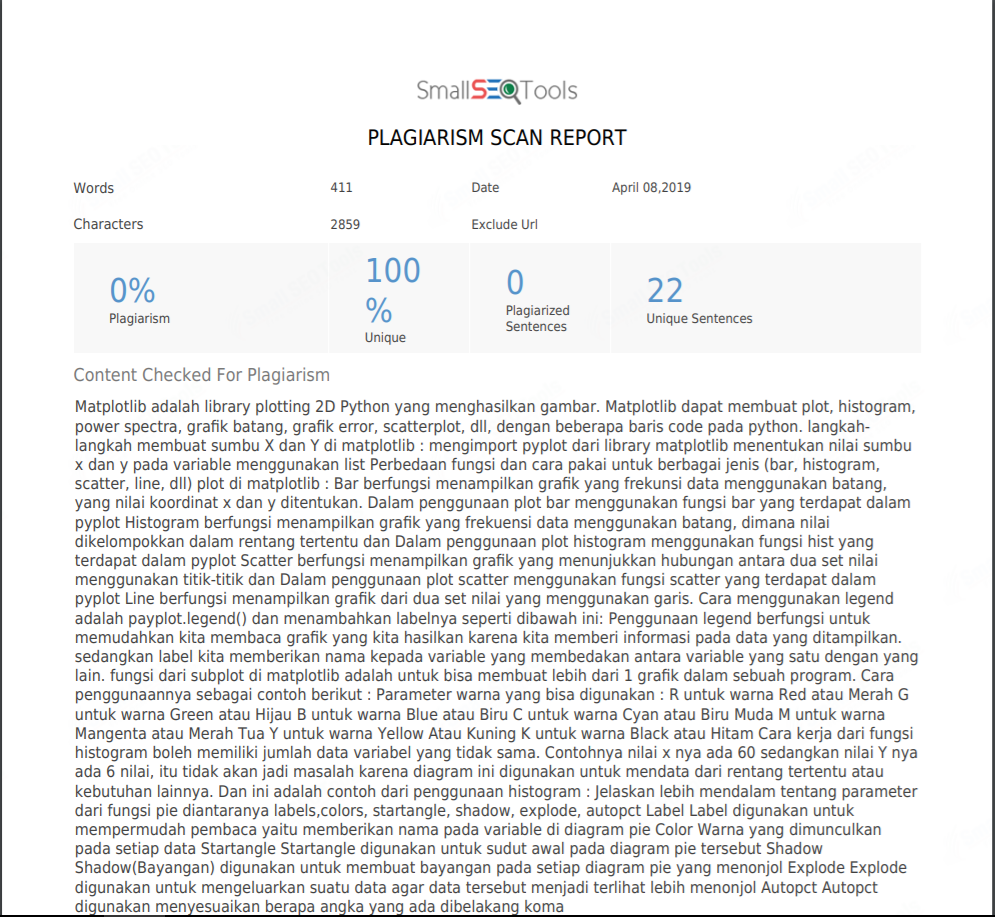
\includegraphics[width=5cm]{figures/6/1174084/Teori/c6_1.png}
    \centering
    \caption{plagiarisme}
    \end{figure}
    
\end{enumerate}
%%%%%%%%%%%%%%%%%%%%%%%%%%%%%%%%%%%%%%%%%%%%%%%%%%%%%%%%%%%%%%%%%%%%%%%%%%%%%